\documentclass[10pt,conference]{IEEEtran}
\IEEEoverridecommandlockouts
% The preceding line is only needed to identify funding in the first footnote. If that is unneeded, please comment it out.
\usepackage{cite}
\usepackage{amsmath,amssymb,amsfonts}
\usepackage{algorithmic}
\usepackage{graphicx}
\usepackage{textcomp}
\usepackage{booktabs}
\usepackage[table,xcdraw]{xcolor}
\usepackage{framed}
\usepackage{float}
\usepackage{xcolor}
\usepackage[hidelinks]{hyperref}
\usepackage{xfrac}

\usepackage{balance}

\usepackage{array}
\newcolumntype{L}[1]{>{\raggedright\let\newline\\\arraybackslash\hspace{0pt}}m{#1}}


\usepackage{listings}

\definecolor{mygreen}{rgb}{0,0.6,0}
\definecolor{lightgreen}{rgb}{0.6,0.9,0.6}
\definecolor{lightyellow}{rgb}{0.9,0.9,0.6}
\definecolor{lightorange}{rgb}{0.9,0.8,0.6}
\definecolor{lightred}{rgb}{0.9,0.7,0.7}
\definecolor{mygray}{rgb}{0.5,0.5,0.5}
\definecolor{lightgray}{rgb}{0.8,0.8,0.8}
\definecolor{mymauve}{rgb}{0.58,0,0.82}


\usepackage{pifont}
\newcommand{\lstbg}[3][0pt]{{\fboxsep#1\colorbox{#2}{\strut #3}}}

\lstdefinestyle{CStyle} {
    language=C,
    backgroundcolor=\color{white},   % choose the background color
    basicstyle=\ttfamily\scriptsize,        % size of fonts used for the code
    breaklines=true,                 % automatic line breaking only at whitespace
    captionpos=b,                    % sets the caption-position to bottom
    commentstyle=\color{mygray}\bfseries,    % comment style
    escapeinside={\%*}{*)},          % if you want to add LaTeX within your code
    keywordstyle=\color{blue},       % keyword style
    stringstyle=\color{mymauve},     % string literal style
    frame=single,
    numbers=left,
    stepnumber=1,
    xleftmargin=2em,
    escapeinside={/*!}{!*/},
    moredelim=**[l][\color{mygreen}]{+\ },
    moredelim=*[l][\color{red}]{-\ }
}

\lstdefinestyle{PHPStyle} {
    language=PHP,
    alsolanguage=HTML,
    backgroundcolor=\color{white},   % choose the background color
    basicstyle=\ttfamily\scriptsize,        % size of fonts used for the code
    breaklines=true,                 % automatic line breaking only at whitespace
    captionpos=b,                    % sets the caption-position to bottom
    commentstyle=\color{mygray}\bfseries,    % comment style
    escapeinside={\%*}{*)},          % if you want to add LaTeX within your code
    keywordstyle=\color{blue},       % keyword style
    stringstyle=\color{mymauve},     % string literal style
    frame=single,
	numbers=left,
    stepnumber=1,
	xleftmargin=2em,
    escapeinside={/*!}{!*/},
    moredelim=**[l][\color{mygreen}]{+\ },
    moredelim=*[l][\color{red}]{-\ }
}


\newcounter{lstannotation}
\setcounter{lstannotation}{0}
\renewcommand{\thelstannotation}{\ding{\number\numexpr181+\arabic{lstannotation}}}
\newcommand{\annotation}[1]{\refstepcounter{lstannotation}\label{#1}\thelstannotation}

\def\BibTeX{{\rm B\kern-.05em{\sc i\kern-.025em b}\kern-.08em
    T\kern-.1667em\lower.7ex\hbox{E}\kern-.125emX}}

%
% Add comments in the text
%
\newboolean{showcomments}
\setboolean{showcomments}{false}
%\setboolean{showcomments}{false}

\ifthenelse{\boolean{showcomments}}
  {\newcommand{\nb}[3]{
  {\color{#2}\small\fbox{\bfseries\sffamily\scriptsize#1}}
  {\color{#2}\sffamily\small$\triangleright~$\textit{\small #3}$~\triangleleft$}
  }
  }
  {\newcommand{\nb}[3]{}
  }

\newcommand\Sof[1]{\nb{Sofia}{red}{#1}}
\newcommand\Luis[1]{\nb{Luis}{mygreen}{#1}}
\newcommand\Rui[1]{\nb{Rui}{blue}{#1}}


\begin{document}

\title{Fixing Vulnerabilities Hinders Maintainability}

\author{
    Anonymou(s) Author(s)

%     \IEEEauthorblockN{1\textsuperscript{st} Given Name Surname}
% \IEEEauthorblockA{\textit{dept. name of organization (of Aff.)} \\
% \textit{name of organization (of Aff.)}\\
% City, Country \\
% email address}
% \and
% \IEEEauthorblockN{2\textsuperscript{nd} Given Name Surname}
% \IEEEauthorblockA{\textit{dept. name of organization (of Aff.)} \\
% \textit{name of organization (of Aff.)}\\
% City, Country \\
% email address}
% \and
% \IEEEauthorblockN{3\textsuperscript{rd} Given Name Surname}
% \IEEEauthorblockA{\textit{dept. name of organization (of Aff.)} \\
% \textit{name of organization (of Aff.)}\\
% City, Country \\
% email address}
}

\maketitle

\begin{abstract}
Security is a requirement of utmost importance to produce software with high
quality. However, there is still a considerable amount of zero-day
vulnerabilities being discovered, and fixed, almost weekly. We suspect that when
developers address these vulnerabilities on their codebases, they actually
affect the maintainability of software, potentially introducing other
vulnerabilities. This paper evaluates the impact of refactorings to improve
security on the maintainability of open-source software. Maintainability is
measured based on the \emph{Better Code Hub}'s model of $10$ guidelines using a
dataset including $607$ security commits. Results show that fixing software
vulnerabilities hinders the maintainability of open-source software. This is
particularly the case for refactorings that address \emph{Broken Authentication
and Session Management} issues, \emph{Memory Leaks} and \emph{Denial-of-Service}
attacks. Furthermore, we conclude that changes to codebases to fix vulnerabilities
need to be performed with extra care.
\end{abstract}

\begin{IEEEkeywords}
Security, Software Maintenance, Open-Source Software
\end{IEEEkeywords}

\section{Introduction}

Software quality is important because it is ultimately related to the overall
cost of developing, extending and maintaining software applications. Software
quality characteristics include, but are not limited to, functional correctness,
reliability, usability, maintainability, and security. Security is an important
non-functional requirement during the development of software systems.  However,
there is still a considerable amount of zero-day vulnerabilities being
discovered, and fixed, almost weekly as disclosed by the Zero Day Initiative
website\footnote{Zero Day Initiative website available at
https://www.zerodayinitiative.com/advisories/published/ (Accessed on \today{})}.
These vulnerabilities are gateways for attackers to penetrate
systems and exploit their resources.
As an example, in the last week of January $2019$, a severe vulnerability in Apple
FaceTime was revealed\footnote{https://thehackernews.com/2019/01/apple-facetime-
privacy-hack.html (Accessed on \today{})} --- the outcome of a design/logical
flaw that allowed callers to see and hear others without them picking up the call.

In $2011$, the International Organization for Standardization (ISO) issued an
update for software product quality ISO/IEC 25010~\cite{iso:2011} considering
\emph{Security} as one of the main software product quality characteristics.
Unmaintainable code is hard to test, analyze and re-use, and thus more difficult
to find vulnerabilities and defects. Therefore, writing maintainable code
prevents the introduction of vulnerabilities in the codebases. In this work, we
are concerned about the impact that patching vulnerabilities may have in the
open-source software maintainability. Are developers affecting software
maintainability when trying to improve software security? We suspect that some
patches may have a negative impact on the software maintainability and
possibly even be the cause of the introduction of new vulnerabilities.

ISO describes software maintainability as ``the degree of effectiveness and
efficiency with which a software product or system can be modified to improve
it, correct it or adapt it to changes in environment, and in requirements'' on
software quality ISO/IEC 25010. As ISO does not provide any specific guidelines
or formula to calculate maintainability, we resort on Software Improvement
Group (SIG)'s web-based source code analysis service Better Code Hub
(BCH)~\cite{Visser:2016:OREILLY} to compute the maintainability of a given
project. There are other well-known standards and models that have been proposed
to increase software security: Common Criteria~\cite{common:2009} which received
negative criticism regarding the costs associated and poor technical evaluation;
the OWASP Application Security Verification Criteria~\cite{oswap:2009} which is
focused only on web applications, and a model proposed by Xu et al. ($2013$)
~\cite{6616351} for rating software security (arguably, it was one of the
first steps taken by SIG to introduce security on their maintainability model).
BCH compiles the ISO/IEC 25010 into a set of $10$ guidelines that are the
base of BCH's evaluation. Two examples are the \emph{Write Simple Units of Code}
based on the McCabe Complexity~\cite{1702388} and \emph{Keep your Codebase Small}
based on the idea that smaller codebases are easier to maintain and less prone to defects~\cite{Visser:2016:OREILLY}.

The particular subject of this paper is to explore whether there is a trade-off
between refactoring source code to patch disclosed vulnerabilities and keeping
(or even improving) the maintainability of software systems. Hedegus et al.
($2018$)~\cite{HEGEDUS2018313}, analyzed the difference of maintainability between
groups of refactored elements and non-refactored and conclude that the source
code elements subjected to refactorings had significantly lower maintainability
than the elements not modified.

In this paper, we present the results of our analysis on the maintainability of
$607$ security changes collected from open-source software, from different
programming languages. The main contributions of the present work are:

\begin{itemize}
	\item An empirical study on the impact of security changes on software
	maintainability and what patterns need more attention.
	\item A replication package with all scripts and data created to perform the
	empirical evaluation, for reproducibility. Available online:
  \url{https://figshare.com/s/3e17518222df6a11a8d6}.
\end{itemize}

This empirical study exhibits proof that changes applied in the codebase to fix
vulnerabilities affect code maintainability. Especially, for refactorings that
address \emph{Broken Authentication and Session Management} issues, \emph{Memory
Leaks} and \emph{Denial-of-Service} attacks. With this study, we intend to highlight
the need for tools to predict the impact of patches on maintainability~\cite{4724577}
and documentation to help developers adopt security best practices~\cite{6311252,
7927935, MESQUIDA201519}.

This paper is structured as follows: section~\ref{sec:motivation} introduces an
example of a security refactoring of a known vulnerability found in
OpenSSL\footnote{Repository available at https://github.com/openssl/openssl
(Accessed on \today{})}; section~\ref{sec:methodology} describes the
methodology used to answer the research questions; section~\ref{sec:results}
presents the results and section~\ref{sec:discussion} discusses their
implications; section~\ref{sec:threats}, threats to the validity of the study
are enumerated; section~\ref{sec:rw} describes the different work and existing
literature in the field of study; and, finally section~\ref{sec:conclusions}
concludes the main findings and elaborates on future work.
%
\section{Motivation and Research Questions}\label{sec:motivation}
%
Due to time-to-market pressure and the lack of security expertise, code-related
security flaws are generally detected \textit{after the fact}, i.e., when
hackers exploit them. It turns out that fixing these issues is as simple as
modifying the software codebase. However, these refactorings may have a negative
impact on software maintenance, mostly because developers follow the quickest
solution to fix the problem and not necessarily the most elegant and performant
one. Thus, we want to understand how security refactorings impact the
maintainability of software.

As an example, consider the refactoring of the Datagram Transport Layer Security
(DTLS) protocol implementation in OpenSSL\footnote{OpenSSL is a toolkit that
contains open-source implementations of the SSL and TLS cryptographic
protocols.} to address a vulnerability where an attacker could cause a Denial-of-Service
(DoS) attack by crafting DTLS handshake messages to trigger memory allocations
corresponding to large length values. This vulnerability is listed at the Common
Vulnerabilities and Exposures dictionary as CVE-$2014$-$3506$\footnote{CVE-$2014$-$3506$
details available at http://cve.mitre.org/cgi-bin/cvename.cgi?name=CVE-2014-3506
(Accessed on \today{})}. It is amongst the vulnerabilities studied in our
evaluation. The following snippet presents the changes performed on the
\emph{ssl/d1\_both.c} file\footnote{CVE-$2014$-$3506$ fix available  at
https://github.com/openssl/openssl/commit/\\1250f12613b61758675848f6600ebd914ccd7636
(Accessed on \today{})} by the OpenSSL developers to patch the vulnerability.

\medskip

\setcounter{lstannotation}{0}
\begin{lstlisting}[style={CStyle}, caption={Fix provided by OpenSSL developers to the
\\CVE-$2014$-$3506$ vulnerability},label={lst:vuln}]
+ static unsigned long dtls1_max_handshake_message_len(const SSL *s){ /*!\annotation{lst:func1}!*/
+  unsigned long max_len = DTLS1_HM_HEADER_LENGTH + SSL3_RT_MAX_ENCRYPTED_LENGTH;
+  if(max_len < (unsigned long)s->max_cert_list)
+     return s->max_cert_list;
+  return max_len;
+ }

  static int dtls1_reassemble_fragment(SSL *s, struct hm_header_st* msg_hdr, int *ok){

// [snip]

- unsigned long frag_len = msg_hdr->frag_len, max_len;
- if((msg_hdr->frag_off+frag_len) > msg_hdr->msg_len)
-    goto err;

- if(DTLS1_HM_HEADER_LENGTH +
-    	SSL3_RT_MAX_ENCRYPTED_LENGTH < s->max_cert_list)
-    max_len = s->max_cert_list;
- else
-    max_len = DTLS1_HM_HEADER_LENGTH +
-   		SSL3_RT_MAX_ENCRYPTED_LENGTH;

+ unsigned long frag_len = msg_hdr->frag_len;

- if((msg_hdr->frag_off+frag_len) > max_len)

+ if((msg_hdr->frag_off+frag_len) > msg_hdr->msg_len ||
+ msg_hdr->msg_len > dtls1_max_handshake_message_len(s))
     goto err; /*!\annotation{lst:func5}!*/

  memset(seq64be,0,sizeof(seq64be));
  seq64be[6] = (unsigned char) (msg_hdr->seq>>8);
  seq64be[7] = (unsigned char) msg_hdr->seq;
  item = pqueue_find(s->d1->buffered_messages, seq64be);
  if(item == NULL)
  {
    frag = dtls1_hm_fragment_new(msg_hdr->msg_len, 1);

// [snip]

 static int
 dtls1_process_out_of_seq_message(SSL *s, struct hm_header_st* msg_hdr, int *ok)
 {

// [snip]

  if(frag_len && frag_len < msg_hdr->msg_len)
     return dtls1_reassemble_fragment(s, msg_hdr, ok);

+ if(frag_len > dtls1_max_handshake_message_len(s))
+    goto err; /*!\annotation{lst:func4}!*/

  frag = dtls1_hm_fragment_new(frag_len, 0);

\end{lstlisting}

Every SSL/TLS connection begins with a handshake which is responsible by the
negotiation between two parties. DTLS provides a mechanism for fragmenting a
handshake message over a number of packets, each of which can be transmitted
separately. In the example (Listing~\ref{lst:vuln}), all functions receive as
input the SSL session, \texttt{s}.\Luis{is the previous sentence relevant?.} In
the \texttt{dtls1\_reassemble\_fragment} function the size of the fragment
\texttt{msg\_hdr-$>$frag\_off+frag\_len} is checked against the handshake
message size \texttt{msg\_hdr->msg\_len} (line $13$) and then against the
maximum size allowed in a DTLS handshake message for \texttt{s} (line
$16$-$21$).\Luis{I'm not sure about my comment: I think it could be easier if
we explain the previous sentence in pure natural language. This kind of
statements \texttt{msg\_hdr-$>$frag\_off+frag\_len} are not easy to process in
this context.} However, it is not verified if \texttt{msg\_hdr->msg\_len} is
lower than the size allowed by DTLS\Luis{did not understand the problem of not
checking the minimum.}. Thus, in line $37$, when \texttt{msg\_len} is allocated
to the fragment buffer, more memory than the allowed might be allocated.
According to the commit message, $10$ handshake messages are allowed per DTLS
connection. Hence, a remote attacker could leverage this issue to trigger
memory allocations corresponding to large length values and lead the system to
memory exhaustion that could end in a DoS attack.\Luis{I'm not happy with this
paragraph. It's difficult to process and I dont think a reviewer will actually
spend a lot of energy to understand this. (Ignore this if you find it clear.)}
The code changes performed to fix the vulnerability were the following:

~\ref{lst:func1} \texttt{dtls1\_max\_handshake\_message\_len} function was
inserted to return the maximum number of bytes allowed in a DTLS
handshake message for \texttt{s}. The minimum is $16$KB but it might be greater if
the maximum certificate list size requires it. More
specifically, it checks if the maximum certificate list size
(\texttt{s-$>$max\_cert\_list}) requires more length than the maximum length
(\texttt{max\_len}). If that condition holds, the function returns the size of
the certificate list, otherwise, it returns the maximum length. This function
replaces lines $18$-$21$.

~\ref{lst:func5} and~\ref{lst:func4} are guards added to different functions to
ascertain that the message and the fragment length are never higher than the
maximum allowed by DTSL. In particular, \ref{lst:func5} is responsible for patching
the vulnerability.

Although checking the maximum size of a handshake message seems an elementary
problem to repair, the example shows that there was a significant amount of
changes performed in the codebase which produced a negative impact in the
maintainability. Even though the developer tries to simplify the
codebase by introducing a smaller unit
\texttt{dtls1\_max\_handshake\_message\_len} (\ref{lst:func1}), this change also
disrupts $2$ of the guidelines proposed by the Software Improvement Group (SIG) for
building maintainable software~\cite{Visser:2016:OREILLY}. It adds a new branch
point to the \texttt{dtls1\_process\_out\_of\_seq\_message} unit
(\ref{lst:func5}) increasing the cyclomatic complexity and breaking the
\emph{Write Simple Units of Code} guideline. Moreover, it increases the codebase
size in $4$ lines of code ($13$ lines added, $9$ lines deleted) which
contributes to a potential violation of the \emph{Keep Your Codebase Small}
guideline. Hence, we have observed that the impact of this refactoring on the
OpenSSL maintainability was negative.

In this paper, our concern is to study whether, while improving software
security, developers are also negatively impacting the maintainability of their
software applications. To answer the following two research questions, we use a
dataset of security refactorings~\cite{Reis:2017:IJSSE} to measure the impact of
the changes in the maintainability of open-source software.

\begin{framed}
\textit{\textbf{RQ1} What is the impact of security refactorings on the
maintainability of open-source software?}
\end{framed}

Often security flaws require refactoring code to make software more secure.
However, there is no evidence yet of how security refactorings impact the
maintainability of open-source software. Our suspicion is that developers tend
to introduce technical debt in their software when refactoring the codebase to
address a security flaw because they tend to choose the easiest path to solve
it. To address it, we compute the maintainability of $607$ commits using
\emph{Better Code Hub}. The same approach is applied to a randomly generated
dataset of regular commits --- baseline --- that we use to understand how
maintainability evolves when security refactorings are performed versus when
they are not.

\begin{framed}
\textit{\textbf{RQ2} Which patterns of security refactorings are more likely to
affect open-source software maintainability?}
\end{framed}

There are security flaws that are more difficult to refactor than others. For
instance, implementing secure authentication is not as easy as fixing a
cross-site scripting vulnerability since usually the last one is can be fixed
without adding new lines of code, as seen in Listing~\ref{lst:fix}. The developer added the function \emph{htmlentities} to
\textit{escape} the data given by the variable \texttt{\$\_['file']}. Knowing which
patterns are more likely to increase maintainability issues is one step forward
to bring awareness to security engineers of what patterns need more attention.
The taxonomy of security patterns used to answer this question is the same as
the one provided by the authors of the dataset~\cite{Reis:2017:IJSSE}.
Maintainability is measured separately for each pattern.

\setcounter{lstannotation}{0}
\begin{lstlisting}[style={PHPStyle}, caption={Fix provided by \texttt{nextcloud/server} developers to a \\Cross-Site Scripting vulnerability},label={lst:fix}]
 <ul>
  <li class='error'>
   <?php echo $l->t('Cloud not found');?>
   <p class='hint'>
    <?php
-   if(isset($_['file'])) echo $_['file']
    ?>
   </p>
   <p class='hint'>
    <?php
+   if(isset($_['file'])) echo htmlentities($_['file'])
    ?>
   </p>
  </li>
 </ul>

\end{lstlisting}

\section{Methodology}\label{sec:methodology}
%
The methodology used to measure the impact of security refactorings on the
maintainability of open-source software is discussed in this section. The
methodology is comprised of the following steps, as illustrated in
Figure~\ref{fig:met}:

\begin{enumerate}
	\item Extract relevant data from a dataset containing $716$ security
	refactorings collected from open-source software available on
	GitHub~\cite{Reis:2017:IJSSE}.
	\item A baseline of regular commits was randomly collected from the list of
	projects of the main dataset to evaluate the impact of regular commits on the
	maintainability of open-source software.
  \item Use the Software Improvement Group's\footnote{SIG's website is available
  at https://www.sig.eu/ (Accessed on \today{})} web-based source code analysis
  service \emph{Better Code Hub} (BCH)\footnote{BCH's website is available at
  https://bettercodehub.com/ (Accessed on \today{})} to quantify maintainability
  for both security and regular commits.
\end{enumerate}

%
\begin{figure}[h]
 	\centering 	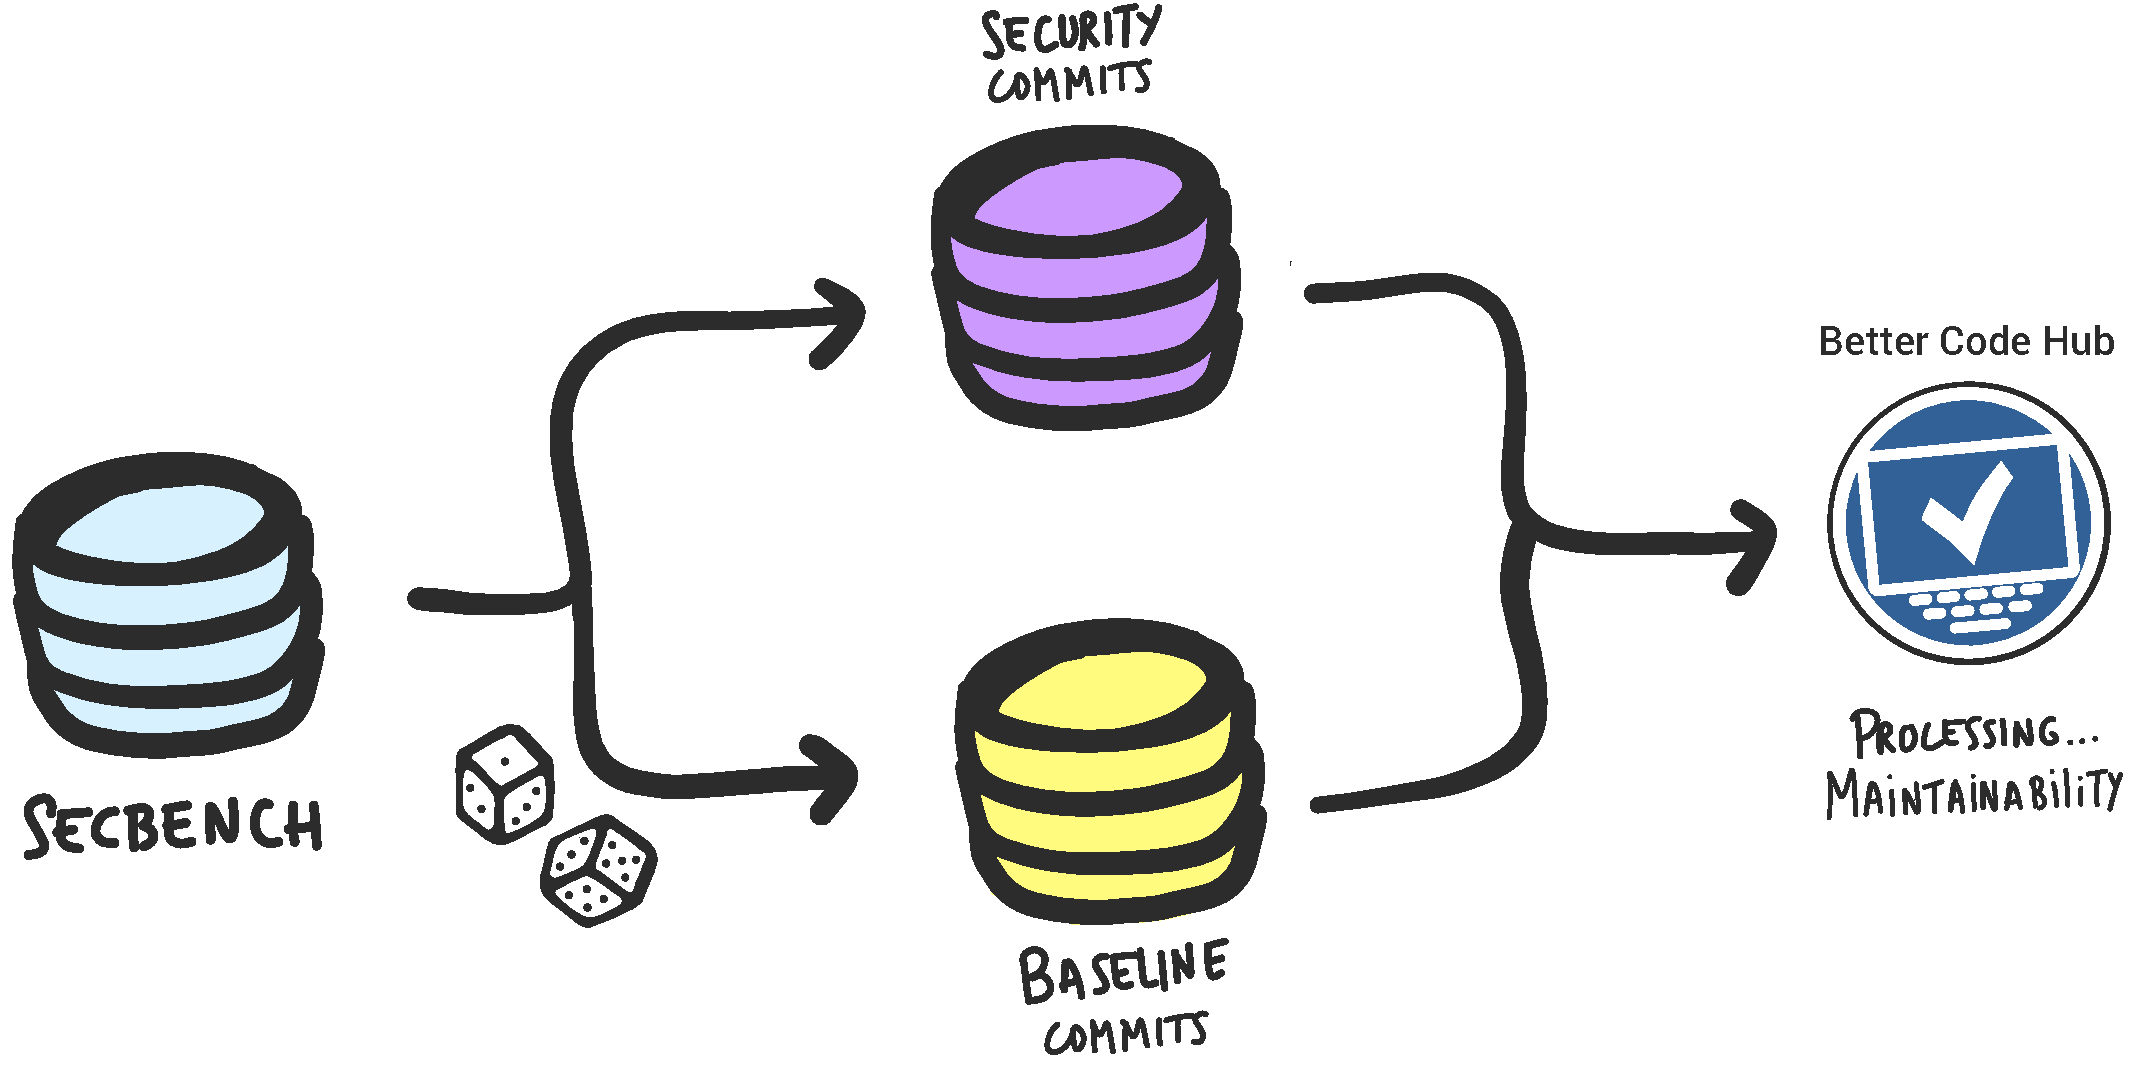
\includegraphics[width=0.4\textwidth]{figures/methodology.pdf}
 	\caption{Study Methodology}
	\label{fig:met}
\end{figure}
%
\subsection{Dataset}
%
To evaluate the impact of security refactorings on the maintainability of
open-source software, we use a dataset of security flaws which is the outcome of
mining $94$ GitHub projects. Reis and Abreu ($2017$) mined open-source
software aiming at the extraction of real examples --- created by real
developers --- to test and assess the performance of static analysis tools since
using hand-seeded test cases or mutations could lead to misleading assessments
of the capabilities of the tools~\cite{just2014mutants}. The study yielded a
dataset with $716$ test cases for $16$ security patterns. Some of the patterns
are based in the OWASP Top $10$ of $2013$~\cite{oswap:2013} and OWASP Top $10$ of
$2017$~\cite{oswap:2017}. Each test case of the
dataset is a triplet: the commit before the refactoring, the commit responsible
for the refactoring, and the snippets of code that differ from one version to
another (typically, called \textit{diffs}) --- where one can easily review the
code used to fix the security flaw. In this study, we focus on computing the
maintainability of the commits before and after the security refactoring to
evaluate if the impact was positive, negative or none.

\begin{figure}[h]
 	\centering 	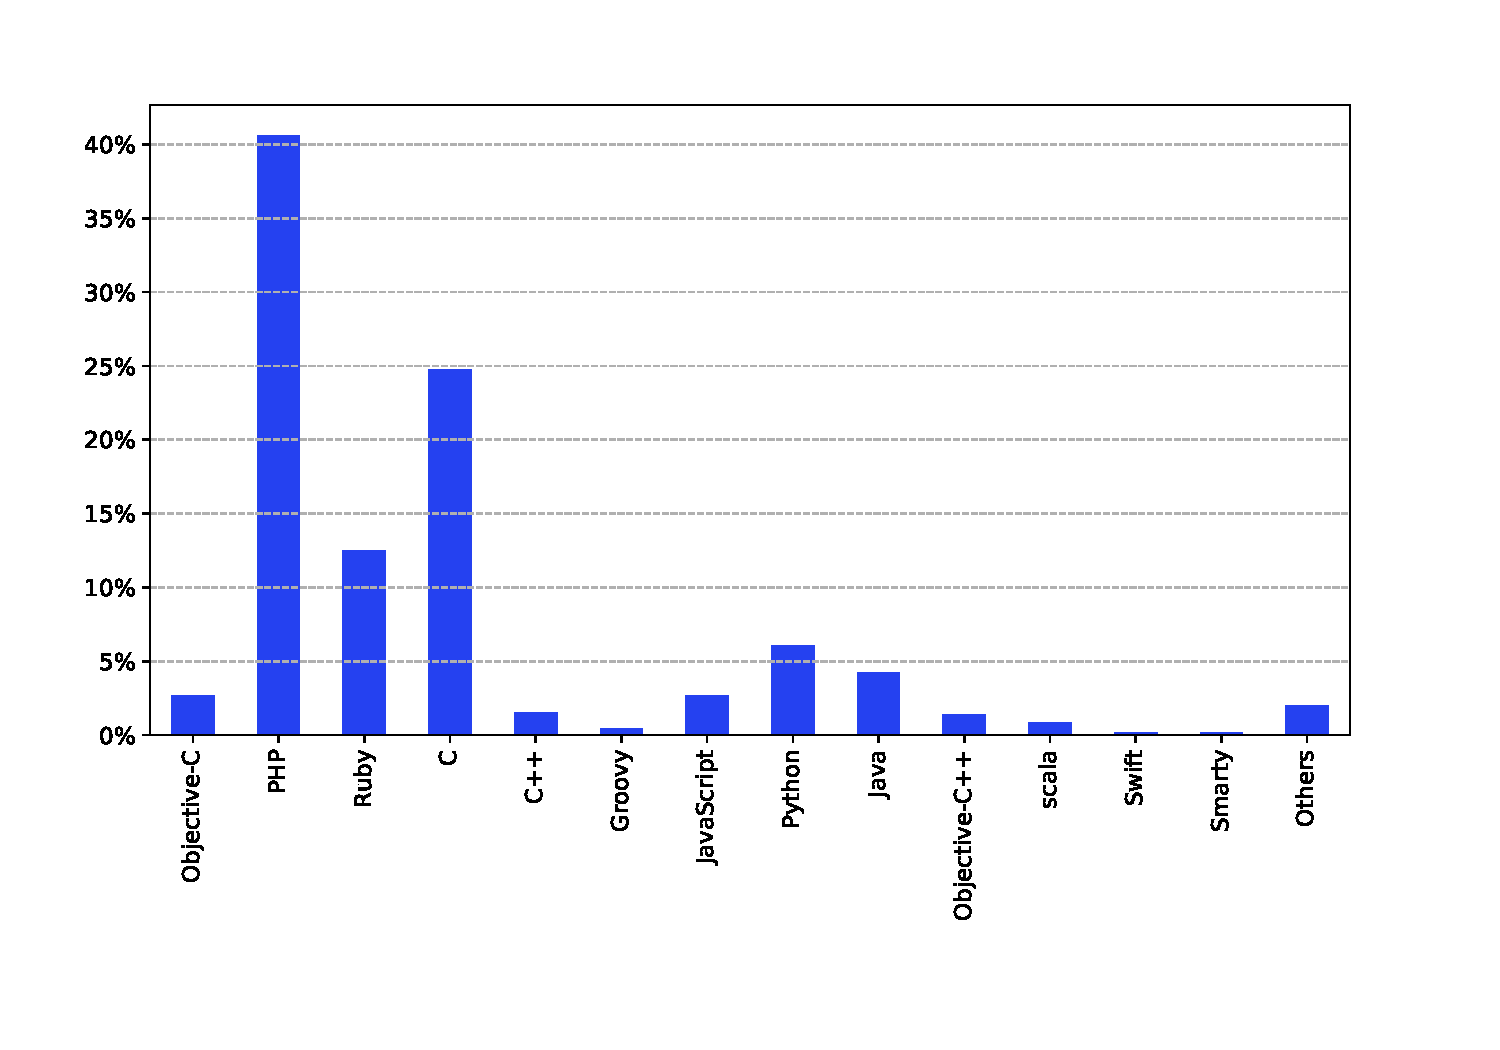
\includegraphics[width=0.4\textwidth]{figures/language_dist.pdf}
 	\caption{Distribution of Security Refactorings per Language\Luis{esta figure pode ser maior nao pode?}}
	\label{fig:lang}
\end{figure}

\begin{figure}[h]
 	\centering 	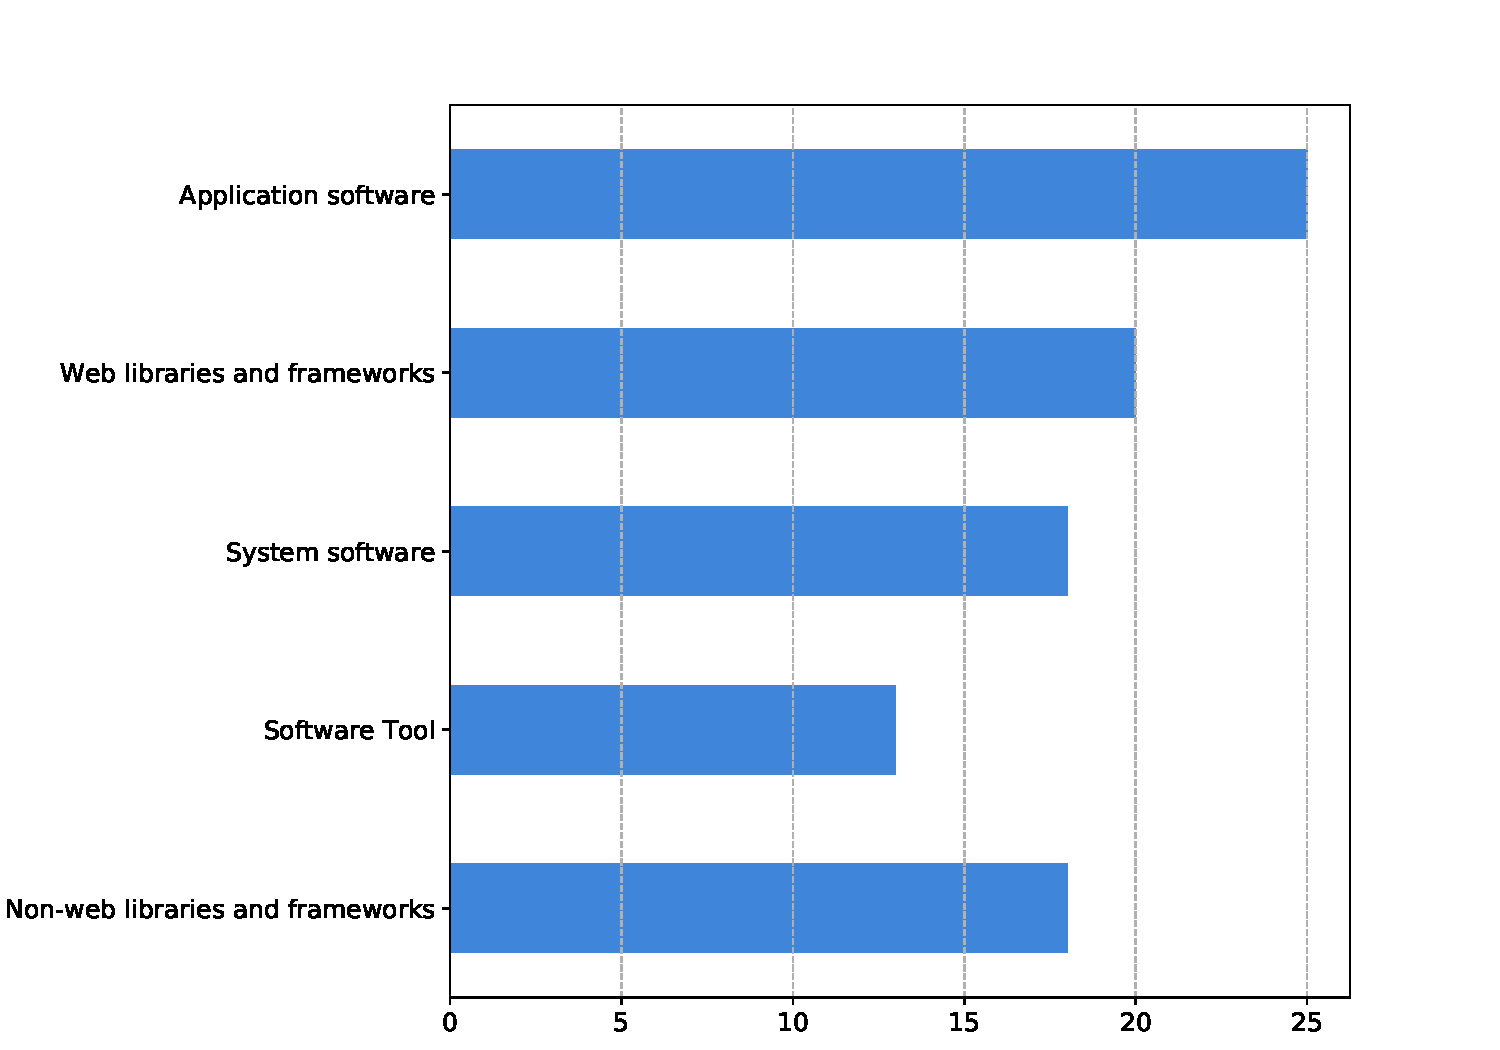
\includegraphics[width=0.4\textwidth]{figures/type_dist.pdf}
 	\caption{Distribution of the Domain of Projects}
	\label{fig:domain}
\end{figure}

The $716$ refactorings in the dataset were run against the BCH toolset to
calculate their maintainability reports. However, there are refactorings
discarded from tour study due to limitations of BCH: in particular, lack of
language support and project size. The final dataset used in this paper contains
$607$ security refactorings labeled as one of the following categories (we
have decided to change the label to \textit{Miscellaneous} of the patterns in
the dataset containing less than $20$ instances):

\begin{itemize}
    \item \textbf{Using Components with Known Vulnerabilities (21 cases).} The majority of
    software produced today integrates several components, such as libraries and
    frameworks, which may affect the software if developers use vulnerable
    versions - usually known and disclosed somewhere on the Internet.
    \textit{Based on the OWASP Top $10$ of $2017$.}

    \item \textbf{Broken Authentication \& Session Management (38 cases).} Incorrectly
    implemented functionalities related to authentication and session
    management, allowing an attacker to gain access to session tokens,
    passwords, keys, and other sensitive data. \textit{Based on the OWASP Top
    $10$ of $2013$.}

    \item \textbf{Cross-Site Request Forgery (30 cases).} Poor session tokens generation
    and management usually allow attackers to send forged HTTP requests
    including authentication information from the victim to the vulnerable web
    application. \textit{Based on the OWASP Top $10$ of $2013$.}

    \item \textbf{Denial-of-Service (40 cases).} Security flaws that can allow an attacker
    to flood or crashing services. This attacks usually occur when the system
    receives much traffic causing it to slow down and eventually stop. For
    example, flaws allowing attackers to trigger memory allocations
    corresponding to large length values (Listing~\ref{lst:vuln}).

    \item \textbf{Cross-Site Scripting (114 cases).} Lack of proper validation or escaping
    allows attackers to submit untrusted data to web browsers through malicious
    scripts that can hijack the user sessions or redirect the user to malicious
    sites. \textit{Based on the OWASP Top $10$ of $2017$.}

    \item \textbf{Injection (89 cases).} When developers do not keep untrusted data
    separate from commands and queries. If an attacker sends a string that
    exploits the syntax of the interpreter, then an injection attack is possible
    (e.g., SQL and LDAP injection). \textit{Based on the OWASP Top $10$ of
    $2017$.}

    \item \textbf{Memory Leak (80 cases).} Memory management issue found more frequently in
    programming languages that do not manage memory automatically (e.g., C/C++
    and Objective-C), i.e., where instead developers are responsible for
    handling it. One of the main causes of DoS attacks.

    \item \textbf{Miscellaneous (195 cases)} This pattern comprises
	several other security refactorings that do not have their own pattern yet and patterns that
	do not satisfy the Wilcoxon test size requirement of more than $20$ refactorings:
    \textit{Resource Leak} (19), \textit{SHA-1 Hash Function} (1),
    \textit{Broken Access Control} (2), \textit{Sensitive Data Exposure} (18),
    \textit{Insufficient Attack Protection} (4), \textit{Overflow} (18),
    \textit{Path Traversal} (19). \end{itemize}

\begin{table*}[h]
	\centering
	\caption{Descriptive statistics of the dataset projects}
\begin{tabular}{@{}rrrrrrrrrrr@{}}
\toprule
      & Forks   & Stars   & Watchers & Contributors & Commits  & Branches & Releases & Size      & Issues & Pull Requests  \\ \midrule
mean  & 1763.52 & 5448.74 & 401.37   & 153.33       & 14834.17 & 45.17    & 129.45   & 122973.24 & 3768.97   & 1941.61 \\
std   & 2434.03 & 6215.09 & 486.60   & 123.68       & 22234.46 & 150.15   & 189.93   & 209732.51 & 5933.16   & 3603.31 \\
min   & 1.00       & 3.00       & 1.00        & 0.00            & 103.00      & 1.00        & 0.00        & 108.00       & 0.00         & 0.00       \\
25\%  & 391.50  & 1581.00    & 117.25   & 49.00           & 1440.50  & 4.00        & 19.00       & 8466.75   & 313.75    & 143.25  \\
median  & 838.50  & 2836.50 & 248.00      & 99.00           & 5504.50  & 9.00        & 59.00       & 37372.50  & 1792.50   & 650.00     \\
75\%  & 2155.00    & 6828.50 & 459.50   & 261.00          & 18579.25 & 20.00       & 142.75   & 117699.50 & 4087.75   & 1907.25 \\
max   & 16366.00   & 31841.00   & 3446.00     & 413.00          & 114378.00   & 1227.00     & 1114.00     & 995790.00    & 33970.00     & 19329.00   \\
Total & 165771.00  & 512182.00  & 37729.00    & 14413.00        & 1394412.00  & 4246.00     & 12168.00    & 11559485.00  & 354283.00    & 182511.00  \\ \bottomrule
\end{tabular}
\label{tab:dataset}
\end{table*}

The dataset contains security flaws for more than $13$ different languages,
being PHP ($39\%$) and C ($24\%$) the most prevalent ones (see Figure~\ref{fig:lang}).
To classify the applications in the dataset, we use a taxonomy for open-source
software from previous work~\cite{7816479}. Figure~\ref{fig:domain}
presents the projects domain distribution: \textit{Application Software} ($25$),
software that provides end-users with functional systems; \textit{Web libraries
and frameworks} ($20$); \textit{System Software} ($18$), software that provides
services and infrastructures (e.g., operating systems, servers and databases);
\textit{Software Tool} ($13$), software that supports development (e.g.,
programming languages, compilers, package managers, IDEs); and, \textit{Non-web
libraries and frameworks} ($18$), for desktop and mobile software.
%
Table~\ref{tab:dataset} presents the descriptive statistics of the $94$
open-source projects involved in this study, including the number of forks, the
number of stars, the number of watchers, the number of contributors, the number
of commits, the number of branches, the number of releases,  size (cf. GitHub, it
is the size of the whole repository, including all of its history, in
kilobytes), the number of issues, and the number of pull requests.


%
\subsection{Security vs. Baseline Commits}
%
Previous studies attempted to measure the impact of regular refactorings on
open-source software maintainability~\cite{HEGEDUS2018313}. However, there is no
previous work focused on comparing the impact of security refactorings with
regular refactorings on maintainability. We analyze the maintainability of
regular commits (i.e., commits not related to security fixes) and use them as a
baseline.

The baseline dataset uses the security commits dataset as input. For each
security commit, one random commit is selected from the list of all commits of
that particular project. We originate the regular commits from the security
commits to ensure that differences in maintainability are not a consequence of
characteristics of different projects.
%
\subsection{Maintainability Analysis}

As said before, the web-based source code analysis service \emph{Better Code
Hub} (BCH) is used to collect the maintainability reports of the refactorings of
each project. Table~\ref{tab:guidelines} presents the $10$ guidelines proposed
by BCH's authors for delivering software that is not difficult to
maintain~\cite{Visser:2016:OREILLY}. During each guideline evaluation, the tool
determines the compliance towards one guideline by establishing limits for the
percentage of code allowed to be in each of the $4$ risk severity levels
(\emph{low risk}, \emph{medium risk}, \emph{high risk}, and \emph{very high
risk}). If the project does not violate the thresholds, then it is compliant
with the guideline. These thresholds are calibrated by BCH using their own
data/experience --- using open-source and closed software systems. If a project is
compliant with a guideline, it means that it is at least $65\%$ better than the
software used by BCH to calculate the thresholds\footnote{Check the answer to
\emph{How can I adjust the threshold for passing/not passing a guideline?} at
https://bettercodehub.com/docs/faq (Accessed on \today{})}.

Figure~\ref{fig:bchrep} shows an example of the report
provided by BCH for a project after finishing its evaluation. The example
refers to the OpenSSL CVE-$2014$-$3506$ vulnerability refactoring ---
as described as motivating example in Section~\ref{sec:motivation}. This
version of OpenSSL only complies with $1$ out of $10$ guidelines: \emph{Write
Clean Code}.

\begin{table}[h]
	\caption{Guidelines to produce maintainable code}
\begin{tabular}{L{2.5cm}L{5.5cm}}

\toprule
\textbf{10 Guidelines} & \textbf{Description}\\
\midrule
\textbf{Write Short Units of Code} & Limit code units to $15$ LOCs because smaller
 units are easier to understand, reuse and test them\\\midrule
\textbf{Write Simple Units of Code} & Limit branch points to $4$ per unit because
it makes units easier to test and modify \\\midrule
\textbf{Write Code Once} & Do not copy code because bugs tend to replicate at
multiple places (inefficient and error-prone)\\\midrule
\textbf{Keep Unit Interfaces Small} & Limit the number of parameters to at most
$4$ because it makes units easier to understand and reuse\\\midrule
\textbf{Separate Concerns in Modules} & Avoid large modules because changes in
loosely coupled databases are easier to oversee and execute\\\midrule
\textbf{Couple Architecture Components Loosely} & Minimize the amount of code
within modules that are exposed to modules in other components\\\midrule
\textbf{Keep Architecture Components Balanced} & Balancing the number of
components ease locating code and allow for isolated maintenance\\\midrule
\textbf{Keep your Codebase Small} & Reduce and avoid the system size because
small products are easier to manage and maintain\\\midrule
\textbf{Automate Tests} & Test your codebase because it makes development
predictable and less risky\\\midrule
\textbf{Write Clean Code} & Avoid producing software with code smells because
it is more likely to be maintainable in the future\\
\bottomrule
\end{tabular}
\label{tab:guidelines}
\end{table}


\begin{figure}[h]
 	\centering 	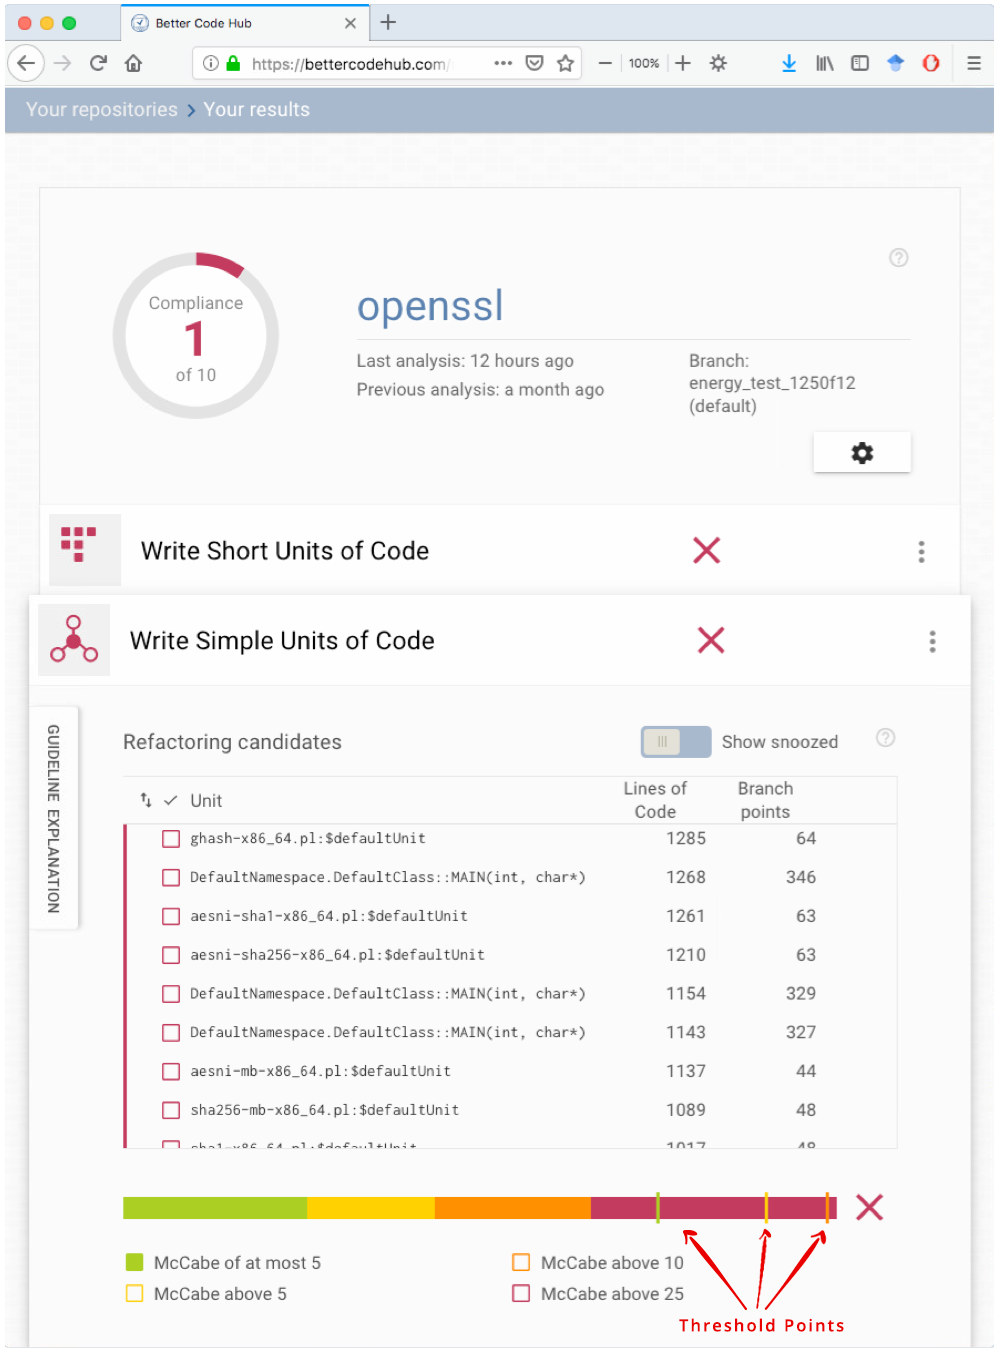
\includegraphics[width=0.4\textwidth]{figures/bch_report.png}
 	\caption{Maintainability report of OpenSSL's CVE-$2014$-$3506$ vulnerability
refactoring for the guideline \emph{Write Simple Units of Code} provided by
\emph{Better Code Hub}. This version of OpenSSL does not comply with the
guideline in the example since the bars do not reach the threshold points. This
example only complies with $\sfrac{1}{10}$ guidelines (\emph{Write Clean Code}).}
	\label{fig:bchrep}
\end{figure}

SIG defines \emph{Units} as the smallest groups of code that can be maintained
and executed independently~\cite{Visser:2016:OREILLY} (e.g., methods and
constructors in Java). One of the guidelines with which the project does not
comply is the one presented in the report (cf. Figure~\ref{fig:bchrep}):
\emph{Write Simple Units of Code}. BCH analyzes this guideline based on the
McCabe Complexity~\cite{1702388} to calculate the number of branch points of a
method. The bar at the bottom of the figure represents the top $30$ units that
violate the guideline, sorted by severity. The violation severities are
indicated using colors, and there is a legend to help to interpret them. The
green bar represents the number of compliant branch points per unit (\emph{at
most $5$}), i.e., the number of units are compliant with ISO
25010~\cite{iso:2011}. Yellow, orange and red bars represent units that do not
comply with medium (\emph{above $5$}), high (\emph{above $10$}) and very high
(\emph{above $25$}) severity levels. In the bar, there are marks that pinpoint
the compliance thresholds for each severity level. If the green mark is
somewhere in the green bar it means it is compliant with a low level of
severity.

\begin{figure}[h]
 	\centering 	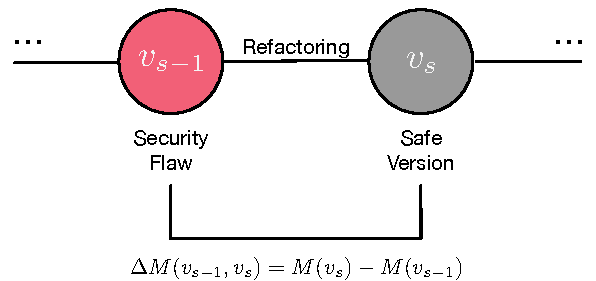
\includegraphics[width=0.49\textwidth]{figures/commit.pdf}
 	\caption{Maintainability difference for security commits}
	\label{fig:commit}
\end{figure}

Aiming to analyze the impact of security refactorings, we use BCH to compute the
maintainability of two different versions of the project (cf. Figure~\ref{fig:commit}):
\begin{itemize}
	\item $v_{s-1}$, the version containing the security flaw, i.e., before the
	refactoring;
	\item $v_{s}$, the version after fixing the security flaw, i.e., after the
	refactoring;
\end{itemize}

The BCH tool does not compute the final score that our study needs to compare
maintainability amongst different project versions. Thus, our work proposes an
equation to capture the distance between the current state of the project and
the standard thresholds based on previous work~\cite{Olivari:2018}. The equation
considers the following:
\begin{itemize}
	\item \textbf{Size of project changes does not affect the maintainability
	difference between two versions, $\Delta M (v_{s-1},v_{s})$.} We
	aim at evaluating security patterns occurring in different projects similarly.
	Thus, the derived metric uses the \textit{raw} number of lines of code rather
  percentages for normalization purposes.
	\item \textbf{Distance to lower severity levels is less penalized than to the
	thresholds in high severity levels.} Severity level weights based on the
	severity level to count lines of code that violate maintainability guidelines.
\end{itemize}

Given the violations for the BCH guidelines, we compute the maintainability score
$M(v)$ as follows:

\begin{equation}
    M(v) = \sum_{g \in G}^{} M_{g}(v)
\end{equation}

\noindent
where $G$ is the group of maintainability guidelines from BCH
(Table~\ref{tab:guidelines}) and $v$ is the version of the software under
evaluation. $M(v) < 0$ indicates that version $v$ is violating (some of) the
guidelines, while $M(v) > 0$ indicates that version $v$ is following
the BCH guidelines.

The maintenance for the guideline $g$, $M_g$ for a given version
of a project is computed with the following equation:

\begin{equation}
    M_{g} = \frac{1}{|L|} \sum_{l \in L}^{} C(l) , L = \{medium, high, veryHigh\}
\end{equation}

\noindent
where $C$ is the compliance with the maintainability guideline for the given
severity level (medium, high, and very high) and $L$ is the group of severity
levels of maintainability infractions. The compliance $C$ for a given severity
level $l$ is derived by:

\begin{equation}\label{eq:3}
    C(l) = LOC_{compliant}(l) - w(l) * LOC_{\neg compliant}(l)
\end{equation}

\noindent
where $LOC_{compliant}(l)$ are the lines of code that comply with the guideline
at the given severity level $l$, $LOC_{\neg compliant}(l)$ are the lines of code
that do not comply with the guideline at the given severity level $l$ and $w(l)$
is the weight factor to heighten the impact of non-compliant lines in comparison to
compliant lines. Finally, the term $w(l)$ is calculated as follows:

\begin{equation}
    w(l) = \frac{1 - T(l)}{T(l)}
\end{equation}

\noindent
where $T(l)$ is the threshold in percentage of the lines of code that are
accepted to be non-compliant with the guideline for the severity level $l$. This
is a standard value defined by BCH. In other words, the factor $w$ is used in
Equation~\ref{eq:3} to highlight the lines of code that are not complying with
the guideline. Then, we compute the difference of maintainability between the
security commit ($v_{s}$) and its parent commit ($v_{s-1}$), as illustrated in
Figure~\ref{fig:commit}.

\subsection{Statistical Validation}\label{sec:statsval}
%
To validate the maintainability differences in different groups of commits
(e.g., baseline and security commits), we use the Paired Wilcoxon signed-rank
test with the significance level $\alpha = 0.05$~\cite{10.2307/3001968}. In
other words, we test the null hypothesis that the maintainability difference
between pairs of versions $v_{v-1}$, $v_v$ (i.e., before and after a
security-commit) come from the same distribution. Nevertheless, this test has a
limitation: it does not consider the groups of commits with a zero-difference
maintainability. In $1959$, Pratt provided an improvement to the test to solve
this issue making the test more robust. Thus, we use a version of the Wilcoxon
test that incorporates the cases where maintainability is different from zero~\cite{10.2307/2282543}.
To understand the effect-size, as
advocated by the Common-language effect sizes\cite{graw:1992}, we compute the
mean difference, the median of the difference, and the percentage of cases that
reduce maintainability.
%
\section{Results}\label{sec:results}

As mentioned before, this study evaluates $607$ security and baseline commits
from $94$ distinct open-source projects, distributed amongst $5$ main
types of software applications. The following section presents the
results obtained for each research question.

\begin{framed}
\textit{\textbf{RQ1} What is the impact of security refactorings on the
maintainability of open-source software?}
\end{framed}

The impact of security and baseline commits in the maintainability of
open-source software is presented in Figure~\ref{fig:secvsreg}. For each type of
change, three types of impact of refactorings in the software maintainability
are presented: \emph{negative}, maintainability decreases (\emph{red});
\emph{none}, maintainability remains the same (\emph{yellow}); and,
\emph{positive}, maintainability increases (\emph{green}). Next to each
type of change, it is shown the mean ($\overline{x}$) and median (M)
of the maintainability difference and the p-value resulting from the
Paired Wilcoxon signed-rank test.

\begin{figure}[h]
 	\centering 	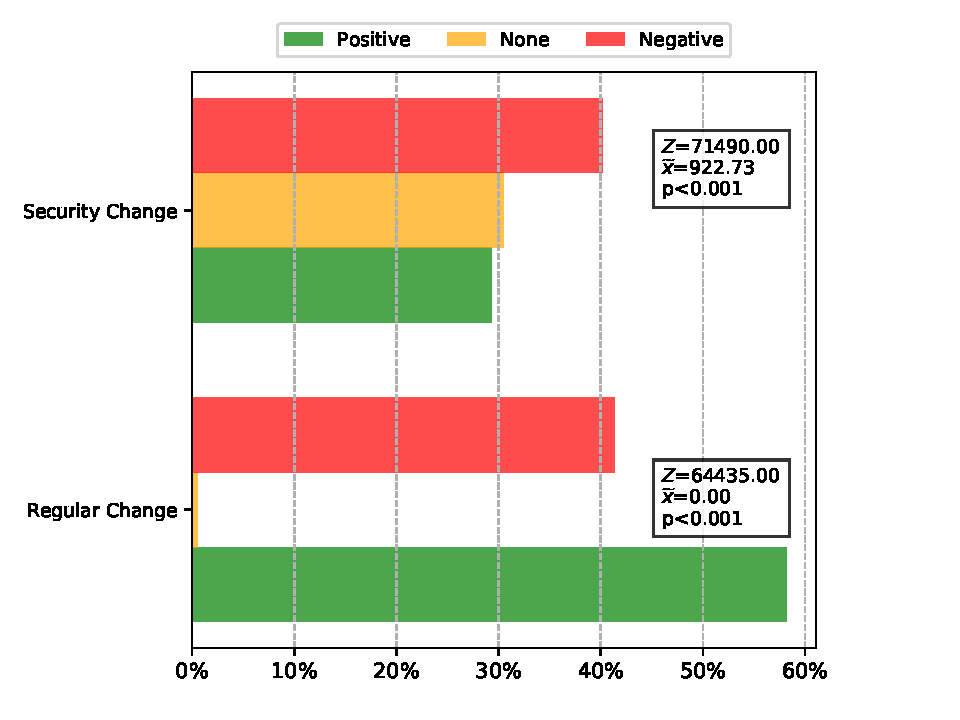
\includegraphics[width=0.5\textwidth]{figures/maintainability.pdf}
 	\caption{Maintainability difference for security and baseline refactorings}
	\label{fig:secvsreg}
\end{figure}

Regarding security commits results, we observe that maintainability decreases in
$40.20\%$ ($244$), remains the same in $30.5\%$ ($185$) and increases in $29.33\%$
($178$) of the cases after security refactorings are applied. The resulting
p-value of the Paired Wilcoxon signed-rank test is $1.21$x$10^{-10}$.
Since the p-value is below the significance level of $0.05$, we argue that
\emph{security refactorings have a negative impact in the maintainability of
open-source software}.

For regular commits, we observe that the maintainability decreases in $41.35\%$
($251$) of the cases after regular refactorings are applied. But in contrast
to security commits, it increases in $58.16\%$ ($353$) and remains the same in
$0.5\%$ ($3$) of the cases. The resulting p-value of the Paired Wilcoxon signed-rank
test is $1.54$x$10^{-6}$. Since the p-value is below the significance level of
$0.05$, we argue that \emph{regular refactorings have a
positive impact in the maintainability of open-source software}.

\begin{figure}[h]
  \centering
  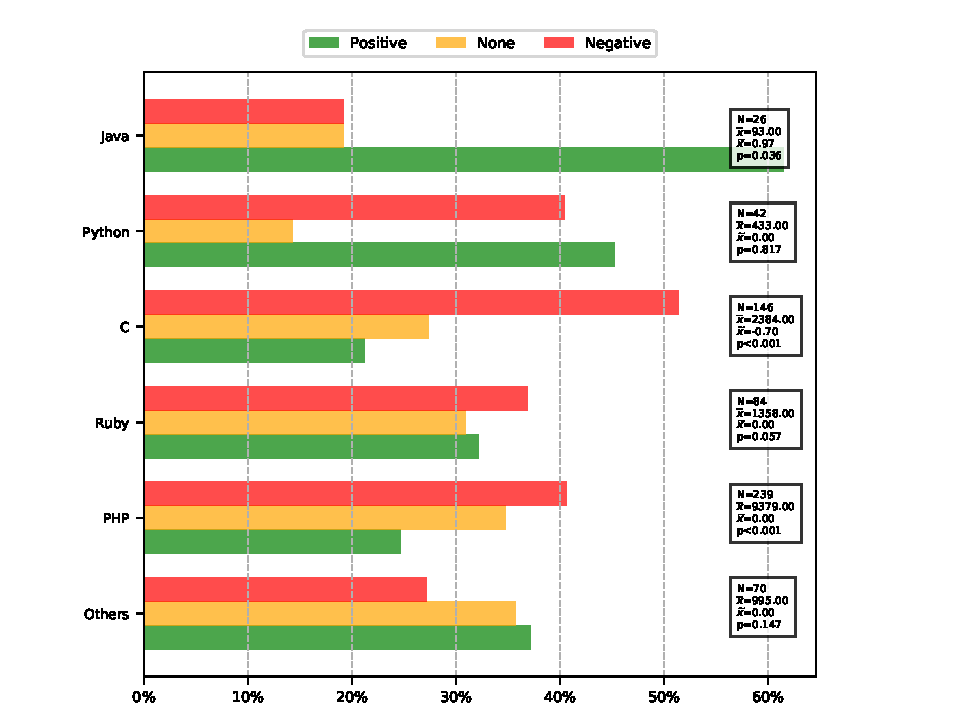
\includegraphics[width=0.45\textwidth]{figures/language.pdf}
  \caption{Maintainability difference by language after security refactorings.}
  \label{fig:lang_main}
\end{figure}

We have also evaluated the impact in the maintainability per programming language
of open-source software, Figure~\ref{fig:lang_main}. Although
the dataset contains security refactorings for more than $13$ languages, we only
present the results for \emph{Java}, \emph{C}, \emph{Ruby}, and \emph{PHP}
because one of the requirements of the Paired Wilcoxon signed-rank is that the
input sample has to have more than $20$ samples. The other languages were
integrated into \emph{Others}. The results of the Paired Wilcoxon signed-rank
test by pattern indicate that there is statistical evidence to support that the
maintainability of open-source software decreases for security refactorings in
$3$ different languages: \emph{C} (p-value = $5.72$x$10^{-9}$), Ruby (p-value = $0.057$) and
PHP (p-value = $3.54$x$10^{-6}$). The results also provide statistical significance
for when security refactorings are performed in \emph{Java} (p-value =
$3.61$x$10^{-2}$). \emph{Python} and the languages that integrate the
\emph{Others} set contain more cases where the maintainability increases.
However, the results obtained for these patterns are not statistically
significant.

\begin{framed}
\textit{\textbf{RQ2} Which patterns of security refactorings are more likely to
affect open-source software maintainability?}
\end{framed}

The impact of each type of security refactoring on the maintainability of
open-source software is presented in Figure~\ref{fig:pat}. The results of the
Paired Wilcoxon signed-rank per pattern indicated statistical
evidence supporting that the maintainability of open-source software decreases
for $4$ different patterns: \emph{Broken Autentication} (p-value = $0.018$),
\emph{Denial-of-Service} (p-value = $0.029$), \emph{Memory Leak} (p-value = $0.009$) and
\emph{Miscellaneous} (p-value = $3.07$x$10^{-4}$). With statistical
significance, results demonstrate evidence that maintainability is not
negatively impacted when removing \emph{Components with Known Vulnerabilities}
(p-value = $7.96$x$10^{-4}$) and fixing \emph{Cross-Site Scripting
Vulnerabilities} (p-value = $0.001$). \emph{Injection} and \emph{Cross-Site
Request Forgery} produced more cases where the refactorings had a negative
impact in the maintainability. However, the results obtained for these patterns
are not statistically significant.

Projects with \emph{Broken Authentication} flaws are the most affected ones by
security refactorings: $55.3\%$ ($21$) of the refactorings had a negative impact
in the maintainability while $35.0\%$ ($11$) yielded a positive impact, and only
$13.8\%$ ($6$) did not suffer any change. The results also show that fixing
\emph{Memory Leak}s affects the maintainability of $51.3\%$ ($41$) of the cases
and leaves only $13.8\%$ ($11$) of the cases unaffected. In $35\%$ ($28$) of the
cases, maintainability increased. Refactoring vulnerabilities that allow
\emph{Denial-of-Service} attacks (e.g., CVE-$2014$-$3506$) have a negative
impact of $47.5\%$ ($19$) in the maintainability of open-source software while
$30.0\%$ ($12$) of the cases exhibit maintainability improvement and $22.5\%$
($9$) show that maintainability does not suffer any change. The
\emph{Miscellaneous} refactorings pattern integrates several types of security
flaws. These type of refactorings harm maintainability in $43.1\%$ ($84$) of the
cases. In $31.8\%$ ($62$), there is no impact and for the
other $25.1\%$ ($49$) maintainability increases.

It is also important to notice that overall the maintainability of open-source
software is not affected by \emph{Cross-Site Scripting} vulnerabilities and by
\emph{Using Components with Known Vulnerabilities}. \emph{Cross-Site Scripting}
does not suffer any decrease in the maintainability of $55.3\%$ ($63$) of cases
and $21.1\%$ ($24$) have a positive effect on it. Only $23.7\%$ ($27$) of the
cases hinder the software maintainability. From the $21$ cases evaluated for
\emph{Using Componentes with Known Vulnerabilities}, only $4.8\%$ ($1$) have a
positive effect in the maintainability of software while $14.3\%$ ($3$) harms
maintainability software, and $81\%$ ($17$) have no effect in the
maintainability.

\begin{figure}[h]
 	\centering
 	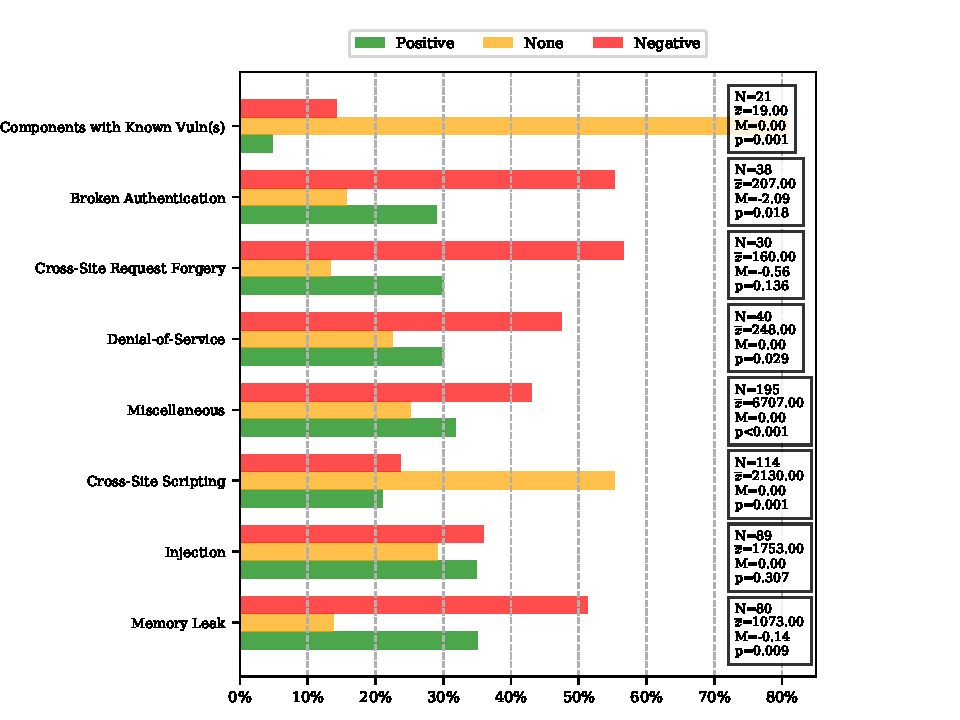
\includegraphics[width=0.50\textwidth]{figures/category.pdf}
 	\caption{Maintainability difference by pattern after security refactorings.
  \Luis{a median e' zero em muitos casos -- como interpretam isso? se nao houver
boa/simples explicacao talvez seja melhor usar o common language.}\Sof{Preciso de pensar melhor nisto}}
	\label{fig:pat}
\end{figure}

\section{Discussion}\label{sec:discussion}

In this section, we discuss the results and answer the proposed research questions.

\begin{framed}
\textit{\textbf{RQ1} What is the impact of security refactorings on the maintainability
of open-source software?}
\end{framed}

\textbf{\textit{Security refactorings harm the maintainability of open-source software.}}
%
We found that $40.2\%$ of the security refactoring have a negative impact on the
maintainability of open-source software (cf. Figure~\ref{fig:secvsreg}). This raises
a new tradeoff when developers need to fix vulnerabilities on their projects
because they might be affecting the software maintainability or even introducing
new vulnerabilities. This study exhibits evidence that developers may have to
reduce maintainability for the sake of security. We understand that developers
should be able to produce secure code without affecting the maintainability of
their projects. But there are still some concerns that need to be addressed:
\begin{itemize}
	\item \textbf{Documentation} of software must provide developers with the
	best practices to implement secure and maintainable software. Unmaintainable
	code is difficult to test, analyze and re-use.

	\item\textbf{Programming Languages} should provide new design patterns to
	easily implement security patterns without endangering maintainability.
	Ultimately, new programming languages, both secure and maintainable by design,
	may be designed to help developers be highly productive when writing and
	maintaining  secure applications. One example is the need for designing new
	authorization mechanisms since these are one of the most complex security
	features to implement.

	\item \textbf{Software Developers} lack the knowledge to create secure and
	maintainable code. Mainly because academic curricula are not yet prepared
	to properly educate them. Universities should do their part on making
	this possible. Online services such as BCH have also a great potential to help
	developers to be more aware of the maintainability issues introduced by their
	changes. Thus, developers can put more work into improving their code maintainability
	and avoid common issues such as code duplication.

\end{itemize}


We would expect that the negative impact of programming languages on
maintainability to be more severe, as arguably poor design of programming
languages and lack of using the best practices lead to more buggy and vulnerable
code~\cite{Ray:2017:LSP:3144574.3126905, 2019arXiv190110220B}. However,
Figure~\ref{fig:lang_main} shows that only \emph{C} has a negative impact of
more than $50\%$ on software maintainability. We suspect that these values are
the result of projects contributions policies. Nine out of ten projects --- the
equivalent to $31.8\%$ of the commits --- of the top-$10$ of dataset projects
with more contributors have restrict contribution policies regarding code
standards. Some examples are the \texttt{laravel/framework},
\texttt{php/php-src}, \texttt{openssl/openssl} and \texttt{cakephp/cakephp}. For
instance, \texttt{laravel/framework} requires the \texttt{PSR-2
Standard}\footnote{PSR-2 Standard available at
https://www.php-fig.org/psr/psr-2/ (Accessed on \today{})}.

\begin{framed}
\textit{\textbf{RQ2} Which patterns of security refactorings are more likely to
affect open-source software maintainability?}
\end{framed}

\textbf{\textit{Broken Authentication \& Session Management, Denial-of-Service
attacks, and Memory Leaks, and Miscellaneous patterns are more likely to affect
open-source software maintainability.}} Although there are a few refactorings
that harm software maintainability in the \emph{Cross-Site Scripting} and
\emph{Using Components with Known Vulnerabilities}, overall maintainability does
not suffer any changes for these patterns. For the remaining patterns,
\emph{Injection} and \emph{Cross-Site Request Forgery}, results are not
statistically significant.

The impact of a refactoring depends on its complexity, i.e., if the refactoring
adds complexity to the codebase it is probably affecting the software
maintainability. One evidence of that is the fact of \emph{Cross-Site Scripting}
and \emph{Using Components with Known Vulnerabilities} refactorings endure more
cases without any impact in the maintainability. Typically, these types of
vulnerabilities do not need extra lines to be fixed, as shown in
Listing~\ref{lst:fix}. Whereas, \emph{Broken Authentication} and vulnerabilities
such as the one presented in Section~\ref{sec:motivation} responsible by Denial-of-Service
attacks are more difficult to fix (several code lines deleted and added).
Another example is the Apple authentication flaw discovered in $2017$
(CVE-$2017$-$13872$)\footnote{CVE-$2017$-$13872$ details available at
https://support.apple.com/en-us/HT208315 (Accessed on \today{})}, where any user
could log in as root with an empty password. Patrick Wardle examined the cause
of the issue\footnote{\emph{Why $<$blank$>$ Gets You Root} available at
https://objective-see.com/blog/blog\_0x24.html (Accessed on \today{})} and
conclude that the flaw was due to the introduction of high cyclomatic complexity
in a method used to verify the password. In sum, \emph{Cross-Site Scripting} and
\emph{Using Components with Known Vulnerabilities} should take part of the
developers' preoccupations along with the other patterns that explicitly hinder
maintainability because despite their low complexity these are patterns that
still produce a considerable negative impact on the maintainability. Real
efforts have been made in creating and incorporating coding standards and best
practices in software production. However, security is still far from perfection
and fixing vulnerabilities might hinder software maintainability. Thus, it is
not only important to provide tool support to developers to help them apply these
patterns without harming software maintainability, but also to create and redesign
programming languages to facilitate developers improving software maintainability.


We measured the effect sizes between both distribution -- before and after
patches --- per language and security patterns using the Common Language Effect
Size~\cite{cliff:1993} method. Effect sizes are of a low-medium level.
Thus, considering the $0$ median and the low effect sizes, it is reasonable
to affirm that there is a significant effect but it might only be
recognized after a thoughtful data analysis.


\section{Threats to Validity}\label{sec:threats}
%
The following section presents the potential threats to the validity of this
study.
%
\subsection{Construct}
%
The maintainability formula was inferred based on the BCH's reports. The high
amount of different projects and backgrounds may require other
maintainability standards. However, BCH does use a representative benchmark of
closed and open-source software projects to compute the
thresholds for each maintainability guideline~\cite{Visser:2016:OREILLY, Baggen2012}.

\subsection{Internal}

The security refactorings dataset provided by the previous
work~\cite{Reis:2017:IJSSE} was collected based on the messages of GitHub
commits produced by project developers to classify the changes performed by them
to fix security flaws. This approach discards security refactorings that were
not explicit in commits messages.

Baseline commits are retrieved randomly by selecting one commit from the same
project of a given security refactoring. This approach softens the differences
that may result from the characteristics of each project. However,
maintainability may still be affected by the developers' experience, coding
style and software contribution policies which is not evaluated in this study.
Furthermore, this evaluation considers that $607$ regular commits are enough to
alleviate random irregularities in the maintainability differences of the
baseline.

\subsection{External}

We use a dataset that only comprises refactorings of open-source software.
However, the methodology requires to access data that is not publicly available.
Thus, our findings may not extend to non-open source software.

Different programming languages may require different coding practices to
address software safety. The dataset comprises more commits in C and PHP, i.e.,
the dataset may not be properly representative of the population regarding
programming languages.

Our approach does not consider security refactorings in any other languages but
English.

\section{Related Work}\label{sec:rw}

Many studies have investigated the relationship between refactorings and
software quality. Previous work focused on object-oriented metrics has evaluated the
impact of refactorings and exhibited proof that quantifying effectively the
impact of refactorings on maintainability may help to choose the appropriate
refactoring type~\cite{1167822}. In contrast to this work, Hegedus et
al.~\cite{HEGEDUS2018313} did not select particular metrics to assess the effect
of refactorings. Instead, statistical tests were used to find the metrics that
have the potential to change significantly after refactorings. The differences
of maintainability between groups of refactored elements and non-refactored were
analyzed. In addition, the authors conclude that the source code elements
subjected to refactorings had significantly lower maintainability than the
elements not affected. Studying the evolution of maintainability issues during
the development of Android apps, Malavolta et al. ($2018$)~\cite{8530041}
discovered that maintainability decreases over time. Palomba et al.
($2018$)~\cite{Palomba:2018:DIM:3231288.3231337} exhibits proof that code smells
should be carefully monitored by programmers since there is a high correlation
between maintainability aspects and proneness to changes and faults. The present
work uses a model proposed by BCH and focuses solely on evaluating the impact of
patching vulnerabilities on software maintainability.

Researchers investigated the relationship between design patterns and software
maintainability~\cite{10.1007/978-3-642-35267-6-18}. $300$ revisions of
\texttt{JHotDraw} were analyzed to conclude that every introduced pattern
instance improved software maintainability. However, other studies show that the
use of design patterns may introduce maintainability issues into
software~\cite{4493325}. The present work studies how security patterns
influence maintainability for open-source software.

There are studies that investigated the impact of programming languages on software
quality~\cite{Ray:2014:LSS:2635868.2635922,Ray:2017:LSP:3144574.3126905}. The first
study shows that some programming languages are more buggy-prone than others. However,
the authors of the second study were not able to reproduce it, not obtaining any
evidence about the impact of language design. Both have used the number of
defects as an indicator of software quality. In addition,
Berger et al. ($2019$)~\cite{2019arXiv190110220B} tried to reproduce~\cite{Ray:2014:LSS:2635868.2635922,
Ray:2017:LSP:3144574.3126905} and identified flaws that throw into distrust the previously demonstrated
correlation between programming language and software defects. Our work studies how
security refactorings affect software quality based on the code maintainability
analysis and provides evidence that programming languages have an impact on
maintainability.

\section{Conclusion and Future Work}\label{sec:conclusions}

This work presents an empirical study on the impact of $607$ security
refactorings on the maintainability of $94$ open-source projects. We leveraged
Better Code Hub reports to calculate maintainability
based on a model proposed in previous work. Security refactorings significantly
affect the software maintainability of open-source software, i.e., developers
hinder maintainability when fixing vulnerabilities. We found this evidence in
$40.2\%$ of the studied cases. Regarding regular commits, it seems that overall
maintainability increases ($50.16\%$). However, there is still a very
considerable amount of cases that harm maintainability ($41.35\%$).

This study also shows evidence that there are security patterns that need more
attention than others. \emph{Broken Autentication} issues,
\emph{Denial-of-Service} attacks and \emph{Memory Leaks} endure maintainability
in $55.3\%$, $51.3\%$, and $47.5\%$, respectively. Therefore, we draw attention
for the need of better documentation explaining how to use best practices to
produce secure and maintainable code; new and better programming languages; new
academic curricula in the fields of security and software quality; and, tools
such as BCH to help developers predict the effect of their patches.

As future work, this study may be extended in many directions: analyze which
guidelines are more likely to be affected by security-related refactorings;
investigate what are the most frequent vulnerabilities in each programming
language; study if there is any correlation between code maintainability and
the popularity of a software project; expand our methodology with other
software quality properties; validate these findings with closed or private
software; and, expand this analysis to other quality standards.



\section*{Acknowledgment}\label{sec:ack}

\noindent
We thank the Software Improvement Group (SIG) team for all the support and
help in validating the methodology.
%ack pedro adao when accepted.

\balance

{
 \bibliographystyle{IEEEtran}
  \bibliography{icpc19}
}

\end{document}
